% DIN-A4 doublesided year calendar
% Author: Robert Krause
% License : Creative Commons attribution license
% Submitted to TeXample.net on 13 July 2012
%\documentclass[landscape,a4paper, magyar, 10pt]{scrartcl}
\documentclass[portrait,a4paper, hungarian, 10pt]{scrartcl}
\usepackage[utf8]{inputenc}
\usepackage[hungarian]{babel}
\usepackage[T1]{fontenc}
\usepackage{tikz} 			% Use the calendar.sty style

\usepackage{translator}	% Hungarian Month and Day names
\usedictionary{my-personal-dictionary}
\usepackage{fancyhdr}		% header and footer
\usepackage{fix-cm}		% Large year in header

\usepackage[portrait, headheight = 2cm, margin=.45cm,
  top = 3.2cm, nofoot]{geometry}
\usetikzlibrary{calc}
\usetikzlibrary{calendar}
\renewcommand*\familydefault{\sfdefault}

% User defined
\def\year{2018}
% Names of Holidays are inserted by employing this macro
\def\termin#1#2{
  \node [anchor=north west, text width= 7cm] at
    ($(cal-#1.north west)+(3em, 0em)$) {\tiny{#2}};
}

%Header
\renewcommand{\headrulewidth}{0.5pt}
\setlength{\headheight}{10ex}
\chead{
  \fontsize{30}{35}\selectfont\textbf{\year}
  \Large\textbf{Naptár}\hfill
}
%Footer
\cfoot{\footnotesize\texttt{http://www.texample.net/}}



\begin{document}
\pagestyle{fancy}
\begin{center}
\begin{tikzpicture}[every day/.style={anchor = north}]
\calendar[
  dates=\year-01-01 to \year-02-28,
  name=cal,
  day yshift = 2 em,
  day code=
  {
    % Ez rajzolja a dobozt a nap számával
    \node[name=\pgfcalendarsuggestedname,every day,shape=rectangle,
    minimum height= .8cm, text width = 8.7cm, draw = gray]{\tikzdaytext};
    % Ez írja a nap nevét translator package dictionary kell a magyarhoz
    \draw (-4.1 cm, -.1ex) node[anchor = west]{\footnotesize%
      \pgfcalendarweekdayshortname{\pgfcalendarcurrentweekday}};
  },
  execute before day scope=
  {
    \ifdate{day of month=1}
    {
      % Shift right
      \pgftransformxshift{9cm}
      % Print month name 
      \draw (0,0)node [shape=rectangle, minimum height= .8cm,
        text width = 8.7cm, fill = lightgray, text= white, draw = red, text centered]
        {\textbf{\pgfcalendarmonthname{\pgfcalendarcurrentmonth}}};
    }{}
    \ifdate{workday}
    {
      % normal days are white
      \tikzset{every day/.style={fill=white}}
      % Vacation (Germany, Baden-Wuerrtemberg) gray background
      \ifdate{between=2016-12-24 and 2016-01-01}{%
        \tikzset{every day/.style={fill=gray!30}}}{}
    }{}
    % Saturdays and half holidays (Christma's and New year's eve)
    \ifdate{Saturday}{\tikzset{every day/.style={fill=red!10}}}{}
    \ifdate{equals=12-24}{\tikzset{every day/.style={fill=red!10}}}{}
    \ifdate{equals=12-31}{\tikzset{every day/.style={fill=red!10}}}{}
    % Sundays and full holidays
    \ifdate{Sunday}{\tikzset{every day/.style={fill=red!20}}}{}
    \ifdate{equals=01-01}{\tikzset{every day/.style={fill=red!20}}}{}
    \ifdate{equals=01-06}{\tikzset{every day/.style={fill=red!20}}}{}
    \ifdate{equals=05-01}{\tikzset{every day/.style={fill=red!20}}}{}
    \ifdate{equals=10-23}{\tikzset{every day/.style={fill=red!20}}}{}
    \ifdate{equals=11-01}{\tikzset{every day/.style={fill=red!20}}}{}
    \ifdate{equals=12-25}{\tikzset{every day/.style={fill=red!20}}}{}
    \ifdate{equals=12-26}{\tikzset{every day/.style={fill=red!20}}}{}
    % Christian holidays
%    \ifdate{equals=2013-03-29}{\tikzset{every day/.style={fill=red!20}}}{}
%    \ifdate{equals=2013-04-01}{\tikzset{every day/.style={fill=red!20}}}{}
%    \ifdate{equals=2013-05-09}{\tikzset{every day/.style={fill=red!20}}}{}
%    \ifdate{equals=2013-05-20}{\tikzset{every day/.style={fill=red!20}}}{}
%    \ifdate{equals=2013-05-30}{\tikzset{every day/.style={fill=red!20}}}{}
  },
 execute at begin day scope=
  {
    % each day is shifted down according to the day of month
    % increase here 
    \pgftransformyshift{-.78*\pgfcalendarcurrentday cm}
  }
];

% Print name of Holidays
%\termin{\year-01-01}{Újév}
%\termin{\year-03-15}{48-as forradalom}
%\termin{\year-05-01}{Munkás Szent József}
%\termin{\year-11-01}{Mindenszentek}
%\termin{\year-12-24}{Szenteste}
%\termin{\year-12-25}{Karácsony 1.\ nap}
%\termin{\year-12-26}{Karácsony 2.\ nap}
%\termin{\year-12-31}{Szilveszter}
\end{tikzpicture}
\end{center}
\end{document}
